% Source: AESP_466_ClassWork/Supplements/Companion/Euler_Sequences_Quaternions/Euler_Sequences_Quaternions.tex

\documentclass[border=4pt]{standalone}
\usepackage{amsmath}
\usepackage{amssymb}
\usepackage{graphicx}
\usepackage{tikz}
\usepackage{xcolor}
\usetikzlibrary{shapes.geometric, arrows.meta, positioning, decorations.pathmorphing, decorations.pathreplacing, patterns, calc, 3d}

\definecolor{Garnet}{HTML}{73000A}
\definecolor{USC_Rose}{HTML}{CC2E40}
\definecolor{USC_Blue}{HTML}{466A9F}
\definecolor{USC_Slate}{HTML}{1F414D}
\definecolor{USC_Olive}{HTML}{65780B}
\definecolor{USC_Lime}{HTML}{CED318}
\definecolor{USC_Gold}{HTML}{A49137}
\definecolor{USC_Black90}{HTML}{565656}
\definecolor{USC_Black10}{HTML}{ECECEC}

\newcommand{\sectionheader}[1]{%
  \vspace{0.5cm}
  {\noindent\Large \textbf{#1}}
  \vspace{0.2cm}
  \hrule
  \vspace{0.1cm}
  \hrule
  \vspace{0.3cm}
}

\begin{document}
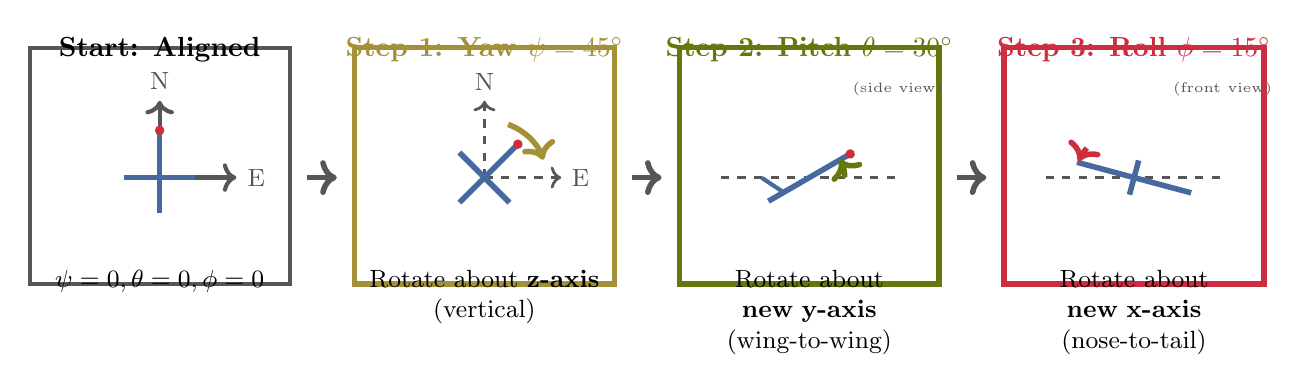
\begin{tikzpicture}[scale=0.75]
    % ===== STEP 0: Starting position =====
    \begin{scope}[shift={(-5.5,0)}]
        \draw[draw=USC_Black90, line width=1.5pt, fill=white] (-2.2,-1.8) rectangle (2.2,2.2);
        \node[above, font=\bfseries] at (0,1.8) {Start: Aligned};

        % Reference axes
        \draw[->, line width=1.5pt, USC_Black90] (0,0) -- (0,1.3) node[above, font=\small] {N};
        \draw[->, line width=1.5pt, USC_Black90] (0,0) -- (1.3,0) node[right, font=\small] {E};

        % Aircraft (top view, pointing north)
        \draw[line width=2pt, USC_Blue] (0,-0.6) -- (0,0.8);
        \draw[line width=2pt, USC_Blue] (-0.6,0) -- (0.6,0);
        \filldraw[USC_Rose] (0,0.8) circle (2pt);

        \node[below, font=\small] at (0,-1.4) {$\psi=0, \theta=0, \phi=0$};
    \end{scope}

    % ===== STEP 1: Yaw rotation =====
    \begin{scope}[shift={(0,0)}]
        \draw[draw=USC_Gold, line width=2pt, fill=white] (-2.2,-1.8) rectangle (2.2,2.2);
        \node[above, font=\bfseries, USC_Gold] at (0,1.8) {Step 1: Yaw $\psi=45^\circ$};

        % Reference axes (fixed)
        \draw[->, line width=1pt, USC_Black90, dashed] (0,0) -- (0,1.3) node[above, font=\small] {N};
        \draw[->, line width=1pt, USC_Black90, dashed] (0,0) -- (1.3,0) node[right, font=\small] {E};

        % Rotation arrow around z
        \draw[->, line width=2pt, USC_Gold] (0.4,0.9) arc (70:20:1.0);

        % Aircraft (top view, rotated 45 degrees)
        \begin{scope}[rotate=-45]
            \draw[line width=2pt, USC_Blue] (0,-0.6) -- (0,0.8);
            \draw[line width=2pt, USC_Blue] (-0.6,0) -- (0.6,0);
            \filldraw[USC_Rose] (0,0.8) circle (2pt);
        \end{scope}

        \node[below, font=\small, text width=3.5cm, align=center] at (0,-1.4) {Rotate about \textbf{z-axis}\\(vertical)};
    \end{scope}

    % ===== STEP 2: Pitch rotation =====
    \begin{scope}[shift={(5.5,0)}]
        \draw[draw=USC_Olive, line width=2pt, fill=white] (-2.2,-1.8) rectangle (2.2,2.2);
        \node[above, font=\bfseries, USC_Olive] at (0,1.8) {Step 2: Pitch $\theta=30^\circ$};

        % Side view indication
        \node[font=\tiny, USC_Black90] at (1.5,1.5) {(side view)};

        % Horizon line
        \draw[line width=1pt, USC_Black90, dashed] (-1.5,0) -- (1.5,0);

        % Aircraft (side view, pitched up)
        \begin{scope}[rotate=30]
            \draw[line width=2pt, USC_Blue] (-0.8,0) -- (0.8,0);
            \filldraw[USC_Rose] (0.8,0) circle (2pt);
            \draw[line width=1.5pt, USC_Blue] (-0.5,0) -- (-0.7,0.4);
        \end{scope}

        % Pitch arc
        \draw[->, line width=2pt, USC_Olive] (0.6,0) arc (0:30:0.6);

        \node[below, font=\small, text width=3.5cm, align=center] at (0,-1.4) {Rotate about \textbf{new y-axis}\\(wing-to-wing)};
    \end{scope}

    % ===== STEP 3: Roll rotation =====
    \begin{scope}[shift={(11,0)}]
        \draw[draw=USC_Rose, line width=2pt, fill=white] (-2.2,-1.8) rectangle (2.2,2.2);
        \node[above, font=\bfseries, USC_Rose] at (0,1.8) {Step 3: Roll $\phi=15^\circ$};

        % Front view indication
        \node[font=\tiny, USC_Black90] at (1.5,1.5) {(front view)};

        % Horizon line
        \draw[line width=1pt, USC_Black90, dashed] (-1.5,0) -- (1.5,0);

        % Aircraft (front view, rolled)
        \begin{scope}[rotate=-15]
            \draw[line width=2pt, USC_Blue] (-1.0,0) -- (1.0,0);
            \draw[line width=2pt, USC_Blue] (0,-0.3) -- (0,0.3);
        \end{scope}

        % Roll arc
        \draw[->, line width=2pt, USC_Rose] (-0.8,0.5) arc (140:155:1.0);

        \node[below, font=\small, text width=3.5cm, align=center] at (0,-1.4) {Rotate about \textbf{new x-axis}\\(nose-to-tail)};
    \end{scope}

    % Arrows between steps
    \draw[->, line width=2pt, USC_Black90] (-3.0,0) -- (-2.5,0);
    \draw[->, line width=2pt, USC_Black90] (2.5,0) -- (3.0,0);
    \draw[->, line width=2pt, USC_Black90] (8.0,0) -- (8.5,0);
\end{tikzpicture}
\end{document}
